% Chapter 4

\chapter{Effective Fermi Hamiltonian} % Main chapter title

\label{Chapter4} % For referencing the chapter elsewhere, use \ref{Chapter3} 

\fancyhead[LO, RE]{Part II. \emph{Kitaev wires}}
\chead{Chapter 4. \emph{Effective Fermi Hamiltonian}} % This is for the header on each page - perhaps a shortened title

%----------------------------------------------------------------------------------------
In this chapter we will derive an effective Hamiltonian for the fermions along the one-dimensional wires. The bosons are asummed to be unaffected, since they live in 3D. Firstly, we calculate the effective pair interaction Hamiltonian for the fermions in section \ref{sec.HFFint}. This is done under the assumption that we can restrict the induced interactions to have a vanishing Matsubara frequency: $\omega_q = 0$. See subsection \ref{sec.RetardationEffects} for the details. In section \ref{sec.meanfieldapproximation} we perform the mean field approximation. The validity of this approach is discussed in section \ref{sec.meanfieldvalidity}. In section \ref{sec.HFFfull} we write up a resulting effective Hamiltonian for the fermions. Here we also diagonalise the Hamiltonian. In section \ref{sec.gapandnumberequations} we derive the gap and number equations. Finally in section \ref{sec.groundstateenergy} we derive an expression for the ground state energy. The approach is an example of a Bardeen-Cooper-Schrieffer (BCS) theory, see e.g. \cite[pp. 359-369]{PlischkeStatPhys}, \cite[pp. 153-163]{LandauStatPhys2} and \cite[chapter 3]{Tinkham}.   

\section{Effective interaction Hamiltonian} \label{sec.HFFint}
The induced interaction between the fermions mediated by the bosons in the condensate result in an effective interaction Hamiltonian for the fermions. In this section we transform the interactions from real to momentum space. 

The \textit{intrawire} interaction Hamiltonian for the effective pair interactions between fermions in wire 1 is given by:
\begin{equation}
H^\text{int,11}_{FF} = \frac{1}{2}\int dx_1dx_2\; \psi^\dagger_{1,F}(x_1)\psi^\dagger_{1,F}(x_2)\tilde{V}^{11}_{\text{ind}}(x_1 - x_2, 0) \psi_{1,F}(x_2) \psi_{1,F}(x_1).
\label{eq.HFF11intdef}
\end{equation}
With $\tilde{V}^{11}_\text{ind}(x,0)$ the induced interaction at zero frequency in real space, equation \eqref{eq.V11indx}. The factor of $1/2$ is present, since the particles are identical. Transforming the above expression to momentum space will make it clearer how to perform the BCS assumption and in turn the mean field approximation. 

The transformation to momentum space is carried out by expanding the field operators in plane waves: $\psi_{1,F}(x) = \frac{1}{\sqrt{\mathcal{L}}}\sum_k \text{e}^{ikx} c_{1,k}$. The transformation is a little tricky, because the induced interaction in momentum space, $V^{11}_{\text{ind}}(p, 0)$, is not well-defined in the zero wire width limit: $l_t = 0$.\footnote{The Yukawa potential simply has no Fourier transform in one dimension.} However, as we shall now see, the direct and exchange term cancel this divergence. This is because the Fermi exclusion principle prohibits identical fermions to be at the same point in space. Formally, we do the following. Firstly:
\begin{align}
\psi_{1,F}(x_2) \psi_{1,F}(x_1) &= \frac{1}{\mathcal{L}}\sum_{k_1,k_2} \text{e}^{i(k_1x_1 + k_2x_2)} c_{1, k_2}c_{1, k_1} = \frac{1}{2\mathcal{L}}\sum_{k_1,k_2} \text{e}^{i(k_1x_1 + k_2x_2)} \left[c_{1, k_2}c_{1, k_1} - c_{1, k_1}c_{1, k_2}\right] \nonumber \\
&= \frac{1}{2\mathcal{L}}\sum_{k_1,k_2} \left[\text{e}^{i(k_1x_1 + k_2x_2)} - \text{e}^{i(k_2x_1 + k_1x_2)}\right]c_{1, k_2}c_{1, k_1}, \nonumber
\end{align}
where we in the last equality switch the momenta in the last term: $k_1 \leftrightarrow k_2$. In this way we take care of the antisymmetry of the fermionic operators. A similar expression for $\psi^\dagger_{1, F}(x_1)\psi^\dagger_{1, F}(x_2)$ is obtained by letting $k_1 \to q_1$ and $k_2 \to q_2$ and taking the hermitian conjugate. All of this is then inserted into the interaction Hamiltonian of equation \eqref{eq.HFF11intdef}. After a little computation, we get:
\begin{align}
H^\text{int,11}_{FF} = \frac{1}{8\mathcal{L}^2} \sum_{k_1,k_2,q_1,q_2} c^\dagger_{1, q_1}c^\dagger_{1, q_2}c_{1, k_2}c_{1, k_1} & \int dx_2 \; \text{e}^{i((k_1 + k_2) -(q_1 + q_2))x_2} \nonumber \\ 
& \cdot \int du\left( \text{e}^{-iq_1u} - \text{e}^{-iq_2u} \right)\left( \text{e}^{ik_1u} - \text{e}^{ik_2u} \right)\tilde{V}^{11}_\text{ind}(u, 0), \nonumber
\end{align}
where we have made the substitution of variables $u = x_1 - x_2$. The integral over $x_2$ is now independent of $\tilde{V}^{11}_{\text{ind}}$. Since we are working with periodic boundary conditions, we get $\int dx_2 \text{e}^{i((k_1 + k_2) - (q_1 + q_2))x_2} = \mathcal{L}\delta_{k_1 + k_2, q_1 + q_2}$ which ensures total conservation of momentum. This means that we can get the above expression on the following form: 
\begin{equation}
H^\text{int,11}_{FF} = \frac{1}{4\mathcal{L}} \sum_{k, q, p} c^\dagger_{1, k + p}c^\dagger_{1, q - p}c_{1, q}c_{1, k} \int du\left[\cos\left(pu\right) - \cos\left(\left( k - q + p \right)u\right)\right]\tilde{V}^{11}_{\text{ind}}(u,0), \nonumber
\end{equation}
where we have made the substitutions: $k_1 = k, k_2 = q, q_1 = k + p$ and $q_2 = q - p$. Finally, since the induced interaction is even in $u$, we have that $V^{11}_{\text{ind}}(p, 0) = \int du \cos(pu) \tilde{V}^{11}_{\text{ind}}(u, 0)$. Due to the antisymmetry of the fermionic particles, the sum of the direct and exchange terms, $W^{11}_{\text{ind}}(k, q, p) = \frac{1}{2}\left( V^{11}_{\text{ind}}\left( p, 0 \right) - V^{11}_{\text{ind}}\left( k - q + p, 0 \right) \right)$, arises as promised in subsection \ref{subsec.inducedinteraction.momentumspace}. The diagrams for these two scattering events are shown in figure \ref{fig.directandexchangediagrams}. This demonstrates diagrammatically that the exchange vertex arises due to the antisymmetry of the fermions. There is a direct term, $V^{11}_\text{ind}\left( p, 0 \right)$, describing a momentum transfer, $p$, and an exchange term, where the fermions exchange their momenta $k$ and $q$, and transfer momentum $p$. We consequently obtain:
\begin{equation}
H^\text{int,11}_{FF} = \frac{1}{2\mathcal{L}} \sum_{k,q,p} W^{11}_{\text{ind}}(k, q, p) c^\dagger_{1, k + p} c^\dagger_{1, q - p} c_{1, q} c_{1, k}. 
\label{eq.H11intMomentumSpace}
\end{equation}
In subsection \ref{subsec.inducedinteraction.momentumspace} we showed that the sum of the direct and exchange terms, $W^{11}_{\text{ind}}$, has a well-defined narrow wire width limit, $l_t \to 0$. Thus the intrawire interaction Hamiltonian has been transformed to momentum space. The interaction of fermions in wire 2 is identically to the above by letting $c_1 \to c_2$.   

\begin{figure}
\center
\begin{tikzpicture}
  \begin{feynman}[small]
    \vertex (number1) {\( \text{Direct} \)};
    \vertex [above left=of number1] (fermion1) {\(1, k \)};
    \vertex [above right=of fermion1] (a);
    \vertex [below right=of a] (fermion2) {\(1, k + p \)}; 
    \vertex [above=1cm of a] (b);
    \vertex [above left=of b] (fermion3) {\(1, q\)};
    \vertex [above right=of b] (fermion4) {\(1, q - p\)};
    \vertex [above=0.5cm of a] (abmiddle);
    \vertex [right=3cm of abmiddle] {\( + \)};
 
    \diagram* {
      (number1) -- [opacity=0.0] (fermion1) -- [fermion] (a) -- [fermion] (fermion2),
      (a) -- [photon, momentum=\(p\)] (b),
      (fermion3) -- [fermion] (b) -- [fermion] (fermion4),
    };
  \end{feynman}
\end{tikzpicture}
\hspace{0.5cm}
\begin{tikzpicture} 
  \begin{feynman}[small]
    \vertex (number1) {\( \text{Exchange} \)};
    \vertex [above left=of number1] (fermion1) {\(1, k \)};
    \vertex [above right=of fermion1] (a);
    \vertex [below right=of a] (fermion2) {\(1, k + p \)}; 
    \vertex [above=1cm of a] (b);
    \vertex [above left=of b] (fermion3) {\(1, q\)};
    \vertex [above right=of b] (fermion4) {\(1, q - p\)};
 
    \diagram* {
      (number1) -- [opacity=0.0] (fermion1) -- [fermion] (a) -- [fermion] (fermion4),
      (a) -- [photon, momentum=\(k - q + p\)] (b),
      (fermion3) -- [fermion] (b) -- [fermion] (fermion2),
    };
  \end{feynman}
\end{tikzpicture}
\caption{The antisymmetry of the fermionic operators leads to a direct vertex, $V^{11}_\text{ind}\left( p, 0 \right)$, and an exchange vertex, $V^{11}_\text{ind}\left( k - q + p, 0 \right)$. In the exchange vertex, the two fermions exchange their momenta $k$ and $q$, and transfer momentum $p$. Separately, the diagrams are divergent in the zero wire width limit, $l_t = 0$. The sum cancels this divergence. } 
\label{fig.directandexchangediagrams}
\end{figure}

Now we turn to the \textit{interwire} interaction Hamiltonian:
\begin{equation}
H^\text{int,12}_{FF} = \int dx_1 dx_2 \psi^\dagger_{1,F}(x_1)\psi^\dagger_{2,F}(x_2) \tilde{V}_{\text{ind}}^{12}(x_1 - x_2,0) \psi_{2,F}(x_2)\psi_{1,F}(x_1).
\label{eq.Hint12realspace}
\end{equation}
Fermions in wire 1 and wire 2 are distinguishable, so the factor of $1/2$ in front is absent. Further, there is no exchange term in this case. Transforming the Hamiltonian to momentum space then simply yields:
\begin{equation}
H^\text{int,12}_{FF} = \frac{1}{\mathcal{L}}\sum_{k,q,p} V_{\text{ind}}^{12}(p, 0) c^\dagger_{1,k + p} c^\dagger_{2, q - p} c_{2, q} c_{1, k}. 
\label{eq.Hint12momentumspace}
\end{equation}
The summand describes a scattering with a momentum exchange $p$ and interwire interaction $V_{\text{ind}}^{12}(p,0)$ given by equation \eqref{eq.V12indq.zerofrequency}. The interwire interaction, $V_{\text{ind}}^{12}(p,0)$, is well-defined in the zero wire width limit, $l_t = 0$. 

\section{BCS approximation} \label{sec.meanfieldapproximation}
Chapter \ref{Chapter3} and section \ref{sec.HFFint} demonstrate that the induced interaction between the fermions mediated by the bosons in the condensate is \textit{attractive}. In this section we will make the BCS mean field approximation, where the attractive interaction leads to pairing of the fermions. 

We again start with the intrawire interaction. First, we assume that only states belonging to opposite momenta couples. This is the usual BCS assumption. This means that we can truncate the sum in equation \eqref{eq.H11intMomentumSpace} to $q = -k$ only. Second, we make a mean field approximation to get the Hamiltonian on a solvable quadratic form. For wire 1, we write:
\begin{equation}
c_{1, -k}c_{1, k} = \braket{ c_{1, -k}c_{1, k} } + \left(c_{1, -k} c_{1, k} - \braket{ c_{1, -k}c_{1, k} } \right) = \braket{ c_{1, -k}c_{1, k} } + A_{11,k}, \nonumber 
\end{equation}
and treat the last part $A_{11,k}$ as a small quantity. In this sense, $\braket{ c_{1, -k}c_{1, k} }$ is an order parameter of the phase transition. We return to this later on. The validity of this approach is discussed in section \ref{sec.meanfieldvalidity}. The mean is the thermal average: $\braket{ c_{1, -k}c_{1, k} } = \tr\left[\text{e}^{-\beta H_{FF}}c_{1, -k}c_{1, k} \right]/Z$ with $Z = \tr\left[\text{e}^{-\beta H_{FF}}\right]$ the partition function. We now only keep terms of $A_{11,k}$ and $A^\dagger_{11,k}$ up to first order. Hence:
\begin{align}
H^\text{int,11}_{FF} = \frac{1}{2\mathcal{L}} \sum_{k, p} W^{11}_{\text{ind}}(k, -k, p) & \left[A^\dagger_{11, k + p}\braket{c_{1, -k}c_{1,k}} + A_{11, k}\braket{c^\dagger_{1, k + p}c^\dagger_{1, -(k+p)}} \right. \nonumber \\
& \left. \phantom{\left[A^\dagger_{11, k + p}\braket{c_{1, -k}c_{1,k}}\right.} + \braket{c_{1, -k}c_{1,k}}\braket{c^\dagger_{1, k + p}c^\dagger_{1, -(k + p)}}\right]. 
\label{eq.H11int.meanfield.firstexpression}
\end{align}
We write $p = k' - k$ and define the effective intrawire induced interaction as:
\begin{equation}
W^{11}_{\text{ind}}(k, k') = W^{11}_{\text{ind}}(k, -k, p = k' - k) = \frac{1}{2}\left(V^{11}_{\text{ind}}\left( k - k', 0 \right) - V^{11}_{\text{ind}}\left( k + k', 0 \right) \right), 
\label{eq.EffectiveInteraction.intrawire}
\end{equation}
with the use of equation \eqref{eq.Wkqp.scattering.amplitude}. The analysis is a BCS treatment as mentioned. However, we will not be assuming any constancy of the effective interaction over a range of momentum, as is the case in traditional BCS-theory \cite[chapter 3]{Tinkham}. Indeed, it is crucial to include the functional form of the effective interaction, $W^{11}_{\text{ind}}(k, k')$, in the analysis as we shall see. Since $V^{11}_{\text{ind}}(q,0)$ only depends on $q^2$, we notice that $W^{11}_{\text{ind}}(k, k')$ is odd in both arguments. Inserting $A_{11,k}$ we can thus bring the above sum on the form:
\begin{equation}
H^\text{int,11}_{FF} = -\frac{1}{2\mathcal{L}}\sum_{k,k'} W^{11}_{\text{ind}}(k, k')\left[ \braket{ c_{1, k'}c_{1, -k'}} c^\dagger_{1,k} c^\dagger_{1, -k} + \braket {c^\dagger_{1, k'}c^\dagger_{1, -k'}} c_{1, k} c_{1, -k} - \braket {c_{1, k'}c_{1, -k'}} \braket {c^\dagger_{1, k}c^\dagger_{1, -k}} \right]. \nonumber
\end{equation}
The same procedure is performed for the fermions in wire 2. We simplify the expression by defining the intrawire pairing potentials:
\begin{equation}
\Delta^{jj}_k = -\frac{1}{\mathcal{L}}\sum_{k'}W^{jj}_{\text{ind}}(k,k')\braket {c_{j, k'}c_{j, -k'}}.
\label{eq.intrawirepairingpotentialdef}
\end{equation}
The intrawire interaction Hamiltonian for fermions in wire 1 and 2 can finally be written as:
\begin{equation}
H^{\text{int},jj}_{FF} = \frac{1}{2}\sum_k \left[\Delta^{jj}_k c^\dagger_{j,k}c^\dagger_{j,-k} + \Delta^{jj *}_k c_{j,-k}c_{j,k} - \Delta^{jj}_k\braket{c^\dagger_{j,k}c^\dagger_{j,-k}} \right].
\label{eq.Hintintrawire.meanfield}
\end{equation}
Since the effective interaction is odd in its arguments, the intrawire pairing potentials are odd as well: $\Delta^{jj}_{-k} = -\Delta^{jj}_k$. This is simply due to the Fermi antisymmetry of identical particles in the same wire. Here it is in order to discuss the naming of $s$- and $p$-wave pairing. In the present thesis we will only use the naming to distinguish between pairings respectively even and odd in $k$. In a more general setup the naming stems from the fact that the pairings come from a partial wave expansion. Hence, there is also $d$-wave pairing, $f$-wave pairing etc. We will not go into any detail with this.

Now we turn to the \textit{inter}wire interaction. As for the intrawire case we assume that only states with opposite momentum couples. Hence, we truncate the sum in equation \eqref{eq.Hint12momentumspace} to $q = -k$ only. Further, we make a mean field approximation with the mean field $\braket{c_{2,k}c_{1,-k}}$. Writing $p = k' - k$ we get:
\begin{align}
H^\text{int,12}_{FF} = \frac{1}{\mathcal{L}} \sum_{k,k'} V_{\text{ind}}^{12}(k - k',0) & \left[\braket{c_{2,k'}c_{1,-k'}}c^\dagger_{1,-k}c^\dagger_{2,k} + \braket{c^\dagger_{1,-k'}c^\dagger_{2,k'}}c_{2,k}c_{1,-k} - \braket{c_{2,k'}c_{1,-k'}}\braket{c^\dagger_{1,-k}c^\dagger_{2,k}} \right]. \nonumber
\end{align}
We therefore define the interwire pairing potential as:
\begin{equation}
\Delta^{12}_k = -\frac{1}{\mathcal{L}} \sum_{k'} V_{\text{ind}}^{12}(k - k',0)\braket{c_{2,k'}c_{1,-k'}}.
\label{eq.interwirepairingpotentialdef}
\end{equation}
As we shall see, this pairing can be of $s$-wave symmetry, since fermions residing in different wires are distinguishable. This brings the interaction part of the interwire Hamiltonian on the following form:
\begin{equation}
H^\text{int,12}_{FF} = \sum_{k} \left[\Delta^{12}_k c^\dagger_{2,k}c^\dagger_{1,-k} + \Delta^{12 *}_k c_{1,-k}c_{2,k} - \Delta^{12}_k\braket{c^\dagger_{2,k}c^\dagger_{1,-k}} \right].
\label{eq.Hintinterwire.meanfield}
\end{equation}
Equations \ref{eq.Hintintrawire.meanfield} and \ref{eq.Hintinterwire.meanfield} are the essential equations for the diagonalisation of the Hamiltonian in section \ref{sec.HFFfull}. The intra- and interwire pairings, $\Delta^{jj}$ and $\Delta^{12}$ respectively, will play a major role in all later analysis. We will see that they describe a tendency to pair up fermions with opposite momenta. 

\section{Validity of the mean field approximation} \label{sec.meanfieldvalidity}
The Mermin-Wagner theorem in the context of superfluidity was first proved by P. C. Hohenberg in 1967 \cite{Hohenberg.MerminWagnertheorem}. It states that there is no true long range order in one and two dimensions. We come with a simplified classical argument that also illuminates how one might circumvent this discouraging fact for a one-dimensional system of fermions. 

Let $\phi$ denote the phase of one of the pairing potentials, $\Delta^{ij}(x)$, in real space. For a truly ordered phase we expect $\phi$ to be constant. If we set this constant to 0, it therefore makes sense to infer a Hamiltonian in powers of $\phi$. The Hamiltonian is assumed not to depend on the phase itself. Therefore, to lowest order in $\phi$, the Hamiltonian associated with a spatially varying phase is: 
\begin{equation}
H[\phi] = \frac{K}{2}\int d^{D}x \; \left(\nabla \phi(x)\right)^2, 
\label{eq.Hphi.maintext}
\end{equation}
in $D$ spatial dimensions. There is no linear term $\nabla \phi$ present, because it vanishes under the integration. In the analysis we will as a start keep $x$ a dimensionless variable. Hence, there is an implicit length scale $\xi_s$. We return to this later on. $K$ is a parameter of unit energy giving the phase stiffness of the system. In appendix \ref{Appendix.longrangeorder.pairingphase} we show that the phase-phase correlation function is then $\braket{ \text{e}^{i(\phi(x)- \phi(x'))} } = \text{e}^{G(x,x') - G(0)}$, where $G(x,x') = \braket{\phi(x)\phi(x')}$ is the two-point correlation function. The means are taken with respect to the underlying Gaussian distribution. Further, we show that:
\begin{equation}
G(x,x') - G(0) = -\frac{1}{\beta K}\int \frac{d^{D}k}{(2\pi)^D}\; \frac{1 - \text{e}^{ikx}}{k^2} = -\frac{|x - x'|}{2\beta K}, \nonumber 
\end{equation}
where the last equality is only valid in one dimension. We introduce the length scale $\xi_s$ by letting $x \to x / \xi_s$. Then the phase-phase correlation function is exponentially damped: 
\begin{equation}
\braket{ \text{e}^{i(\phi(x)- \phi(x'))} } = \text{e}^{G(x,x') - G(0)} = \text{e}^{-\frac{|x - x'|}{2\beta K \xi_s}}. 
\label{eq.phasecorrelationfunction.onedimension.maintext} 
\end{equation}
This expresses that there is no true long range order in $D = 1$ dimensions. More specifically we can say that the phase fluctuations associated with the Hamiltonian \eqref{eq.Hphi.maintext} destroys the long range order.\footnote{In one dimension it does so in an exponential way. In two dimension it decays with a power law. Only in three dimensions (and higher) does true long range order prevail.} We will later see that the mean field theory predicts an energy gap in the spectrum. This gap and in turn the resulting superfluidity is in essense due to the spontaneous breaking of a continuous symmetry, namely the choosing of a specific phase of the pairing \cite[pp. 341-346]{BruusFlensberg}. However, the above analysis shows that if the exponential decay is on a microscopic scale no specific phase of the pairing is actually chosen and hence no superfluidity. 

This sounds quite discouraging. However, the above analysis also proposes a loophole: what if $\xi_s$ is macroscopically large? Then the decay of the correlation function is, albeit exponential, on a macroscopic scale. One then talks of quasi long range order. There is one parameter we may suspect is linked to the length scale $\xi_s$. This is the range of the induced interaction; the BEC coherence length $\xi$. Hence, we might be able to reach a macroscopic length scale for the phase fluctuations of the pairing field by making the coherence length sufficiently large. This is in part supported by recent work by Ortiz and Cobanero. They investigate an exactly solvable model in one dimension which has a real space interaction that drops off as $1 / r$, $r$ being the interparticle distance \cite{Ortiz.Beyondmeanfieldtheory}. This is also the behaviour of the Yukawa interaction we consider in the infinite range limit, $\xi \to \infty$. Ortiz and Cobanero show that their model supports a gap opening, and hence the system must be ordered on a macroscopic scale. In another article Ortiz investigates an analogous two-dimensional system, also with a $1 / r$ dependency of the interaction which is also exactly solvable \cite{Ortiz.pxpy}. Here they find that the mean field results fit beautifully with their exact solution.

We may therefore speculate that since the interaction in the present context can also be made long range by going to large coherence lengths, the superfluid phase is not destroyed in one dimension. Further, we may speculate that the analysis based on the mean field approximation will be \textit{qualitatively} correct in the long coherence length limit, $k_F\xi \gg 1$. We can also argue for this in an intuitive way. In the long range limit, the fermions interact with a macroscopic number of particles. Hence, going to lower dimensions does not necessarily mean that the fermions also have fewer neighbours. We simply have to enhance the interaction range, $\xi$. Since the model in the present context is not exactly solvable\footnote{At least not to the authors knowledge.}, the only reasonable way to investigate these speculations is to investigate the fluctuations of the order parameters $\braket{c_{i,-k}c_{j,k}}$. However, we have no way of determining these fluctuations within mean field theory. It therefore remains an open question whether the approach is applicable. We consider it a possible and highly interesting topic of future work. 

In the long coherence length limit, $k_F\xi \gg 1$, we can no longer ignore retardation effects, because the Bogoliubov excitations in the BEC are slowed down: $\frac{v_F}{c_0} = \frac{m_B}{m_F}\frac{k_F\xi}{\sqrt{2}} > 1$. However, as mentioned in the end of chapter \ref{Chapter3}, the induced interaction for nonzero Matsubara frequencies is qualitatively the same as the zero frequency component\footnote{See appendix \ref{Appendix.inducedinteraction.realspace} for the derivation of the general real space interaction.}. Hence, including these effects will not make a qualitative difference.

It is also possible that the work we precent is qualitatively sound, even though the energy gap might close. Sau et al. have shown, how one can address pairing of fermions in number conserving systems in one dimension using the Luttinger liquid formalism \cite{Flensberg.numberconserving1Dfermions}. In the system they consider, they find long-range order of a specific phase, even though the superfluid phase has no such long range order. This work has been extended by Kane et al. and Ruhman and Altman in two recent articles \cite{Kane.Pairing.Luttingerliquids, Altman.Pairing.spinlessfermions}. For the systems they look at, they find a gapless weak coupling and gapped strong coupling phase. They conclude that these are in a one-one correspondence to the weak and strong coupling phases of systems without number conservation. Specifically, there is a topological phase transition between the two phases. It is exactly this behaviour we will find using the mean field approach.

There are mainly two reasons, why we would like to be able to use the mean field approach. Firstly, this approximation approach is by far the simpler one. Secondly, the topological classification dubbed the tenfold way is developed for band Hamiltonians \cite{Ryu.Topology}. There is no fully developed classification scheme for interaction Hamiltonians. We will continue on with the mean field approach encouraged by the result of Ortiz and Cobanero and by the large amount of work done in one dimensional superfluid systems, see e.g. articles \cite{Alicea, KitaevTopPhases, KitaevQuantumWires, LiYangChen, FuKane2006, GreiterIsingKitaevChain, DeGottardiMajoranaFermions, BudichTopInvMajoranaWires}. 

\section{Effective BCS Hamiltonian} \label{sec.HFFfull}
We will now write down the effective BCS Hamiltonian for the fermions. The free particle Hamiltonian for the fermions is: $H_{0,1} + H_{0,2} = \sum_{j,k}\frac{k^2}{2m_F}c^\dagger_{j,k}c_{j,k}$, giving the kinetic energy of the fermions. When the interaction part is treated within BCS theory, it is not number conserving, since it contains terms like $c^\dagger c^\dagger$. Instead we impose diffusive equilibrium by subtracting $\mu_1N_{1,F}+\mu_2N_{2,F}$. $\mu_j$ is the chemical potential of wire $j$ and $N_{j,F} = \sum_k c^\dagger_{j,k}c_{j,k}$ is the number operator for the $j$ fermions. We consequently get the following Hamiltonian:
\begin{align}
H_{FF} = &\sum_j \left[H_{0,j} - \mu_j N_{j,F}\right] + H^\text{int}_{FF,11} + H^\text{int}_{FF,22} + H^\text{int}_{FF,12} \nonumber \\
       = &\frac{1}{2}\sum_k C^\dagger_k \mathcal{H}_{FF,k}C_k + \tilde{\Phi}, 
\label{eq.BCSHamiltonian}
\end{align}
where $\tilde{\Phi} = \frac{1}{2}\sum_k\left[\varepsilon_{1,k} + \varepsilon_{2,k} - \Delta^{11}_k\braket{c^\dagger_{1,k}c^\dagger_{1,-k}} - \Delta^{22}_k\braket{c^\dagger_{2,k}c^\dagger_{2,-k}} - 2\Delta^{12}_k\braket{c^\dagger_{2,k}c^\dagger_{1,-k}} \right]$ is an energy constant related to the ground state energy and with:
\begin{equation}
\mathcal{H}_{FF,k} = \begin{bmatrix} \varepsilon_{1,k} & \Delta^{11}_k      & 0                 & -\Delta^{12}_{-k} \\ 
                                     \Delta^{11 *}_k   & -\varepsilon_{1,k} & \Delta^{12*}_k    & 0 \\ 
                                    0                  & \Delta^{12}_k      & \varepsilon_{2,k} & \Delta^{22}_k \\ 
                                     -\Delta^{12*}_{-k}& 0                  & \Delta^{22*}_k    & -\varepsilon_{2,k} \end{bmatrix}, \hspace{0.5cm}
C_k =  \begin{bmatrix} c_{1,k} \\ c^\dagger_{1,-k} \\ c_{2,k} \\ c^\dagger_{2,-k} \end{bmatrix}.                                     
\end{equation}
Here $\varepsilon_{j,k} = \frac{k^2}{2m_F} - \mu_j$ is the kinetic energy relative to the chemical potential of fermions in wire $j = 1, 2$. This has a quite general structure. We assume that the number of fermions in each wire is the same which means $\mu = \mu_1 = \mu_2$. Hence, we let $\varepsilon_{j,k} \to \varepsilon_k$. Secondly, we make two separate gauge transformations to make the intrawire pairings, $\Delta^{jj}$, real. This works in the following fashion. We assume that the phase of the intrawire pairings are global, i.e. not dependent on the $k$. Hence, we let $\Delta^{jj} \to \Delta^{jj} \text{e}^{i\phi^{jj}}$, with $\text{e}^{i\phi^{jj}}$ the phase of the pairing. We then make the gauge transformation $c_{j,k} \to \text{e}^{-i\phi^{jj}/2}c_{j,k}$. From equation \eqref{eq.intrawirepairingpotentialdef} the intrawire pairing is linearly dependent on $\braket{c_{j,k}c_{j,-k}}$. Hence, under this gauge transformation we get:
\begin{equation}
\Delta^{jj}_k \text{e}^{i\phi^{jj}} \to \text{e}^{-i\phi^{jj}}\Delta^{jj}_k \text{e}^{i\phi^{jj}} = \Delta^{jj}_k, \nonumber
\end{equation}
whereby the intrawire pairings are real. Since the chemical potential is the same for the two wires, they are equivalent. Hence, the system is symmetric in the fermions belonging to wire 1 and 2. In turn the pairings must be equal up to an overall phase: $\Delta^{22}_k = \text{e}^{i\phi} \Delta^{11}_k$. Since they are now real we can obtain the relation: $\Delta^{22}_k = -\Delta^{11}_k$. The overall sign difference is chosen, since it makes the eigenvectors to $\mathcal{H}_{FF,k}$ a bit simpler. The system consists of two distinguishable types of fermions, one belonging to wire 1 the other to wire 2. Hence, we should be able to think of the fermions in wire 1 as spin up and the fermions in wire 2 as spin down. Labeled with such a pseudospin the interwire pairing is expected to be $s$-wave type. We will therefore search for an even solution of $\Delta^{12}_k$. This means that:
\begin{equation}
\mathcal{H}_{FF,k} = \begin{bmatrix} \varepsilon_{k}   & \Delta^{11}_k      & 0                 & -\Delta^{12}_{k} \\ 
                                     \Delta^{11}_k     & -\varepsilon_{k}   & \Delta^{12*}_k    & 0 \\ 
                                    0                  & \Delta^{12}_k      & \varepsilon_{k}   & -\Delta^{11}_k \\ 
                                     -\Delta^{12*}_{k} & 0                  & -\Delta^{11}_k     & -\varepsilon_{k} \end{bmatrix}.     
\label{eq.Hamiltoniankernelmomentumspace}                                                  
\end{equation}
We have hereby specified two global phases. The interwire pairing, $\Delta^{12}_k$, is linearly dependent on $\braket{c_{2,k}c_{1,-k}}$. This means that if we change the phase of the interwire pairing, the relative phase of $\Delta^{11}$ and $\Delta^{22}$, i.e. of $\braket{c_{1,k}c_{1,-k}}$ and $\braket{c_{2,k}c_{2,-k}}$, changes as well. However, this we already fixed to $\Delta^{22}_k = - \Delta^{11}_k$. We have therefore utilized the full gauge freedom of the Hamiltonian which means that the phase of $\Delta^{12}$ must be held completely general for the time being. We notice that for $\Delta^{12} = 0$, the Hamiltonian consists of two independent blocks of Kitaev Hamiltonians, as is evident from comparing the above to equation \ref{eq.HKitaevpre}. This means that the above Hamiltonian describes interacting Kitaev wires. 

The diagonalisation of equation \eqref{eq.BCSHamiltonian} is now in principle straightforward, but quite lengthy due to the $4\times 4$ structure of the matrix kernel in equation \eqref{eq.Hamiltoniankernelmomentumspace}. The eigenvalues of $\mathcal{H}_{FF,k}$ above come in plus/minus pairs. The norm of the eigenvalues give the energy dispersion: 
\begin{equation}
E^{\pm}_{F,k} = \sqrt{\varepsilon_k^2 + |\Delta^{11}_k \pm \Delta^{12}_k|^2} = \sqrt{\varepsilon^2_k + \left(\Delta^{11}_k\right)^2 + \left|\Delta^{12}_k\right|^2 \pm \Delta^{11}_k(\Delta^{12}_k + \Delta^{12*}_k)}
\end{equation} 
This shows that the excitation energies depends on the phase of the interwire pairing, $\Delta^{12}_k$. Since $\Delta^{11}_k$ is odd in $k$ and $\Delta^{12}_k$ is even in $k$, we get that $E^{+}_{F,k} = E^{-}_{F,-k}$. Notice that due to the presence of $\pm \Delta^{11}_k(\Delta^{12}_k + \Delta^{12*}_k)$ in $E^{\pm}_{F,k}$, the dispersions are neither even nor odd in $k$. If one is bothered by this, it is possible to redefine the eigenvalues to $\bar{E}^{\pm}_{F,k} = \sqrt{\varepsilon^2_k + \left(\Delta^{11}_k\right)^2 + \left|\Delta^{12}_k\right|^2 \pm |\Delta^{11}_k(\Delta^{12}_k + \Delta^{12*}_k)|}$ which are manifestly even in $k$. This is a basic reshuffling of the eigenvalues since $E^{\pm}_{F,k}$ are degenerate in $k = 0$. The eigenvectors are however much more involved, and in turn the derivation of the gap equations is more cumbersome. The result in the end is the same however, and therefore we will stick to the above energy eigenvalues. The energy dispersions are plotted in figure \ref{fig.Dispersionexamples} in the two cases: imaginary and real interwire pairing, $\Delta^{12}_k$. We will later see that these two cases are of special interest. For an imaginary interwire pairing the two energy dispersions, $E^{\pm}_{F,k}$, are completely degenerate. This is shown to the left. For a real interwire pairing, they are only degenerate in $k = 0$. $E^{+}_{F,k}$ is close to zero at $k = -k_F$, $E^{+}_{F,k}$ at $k = +k_F$. This is shown to the right. In this figure we have simply set $\mu = \epsilon_{F,0}$, $\Delta^{11}_k / \epsilon_{F,0} = 0.3 k / k_F$ linear, and $\Delta^{12}_k / \epsilon_{F,0} = 0.1$ constant. We expect this behaviour of the pairings for $k / k_F \ll 1$. In the numerical analysis we will see that the pairings in fact decay to 0 for large $k / k_F$ due to the $k$-dependency of the induced interactions. 

\begin{figure} 
\begin{center}  
% GNUPLOT: LaTeX picture with Postscript
\begingroup
  \makeatletter
  \providecommand\color[2][]{%
    \GenericError{(gnuplot) \space\space\space\@spaces}{%
      Package color not loaded in conjunction with
      terminal option `colourtext'%
    }{See the gnuplot documentation for explanation.%
    }{Either use 'blacktext' in gnuplot or load the package
      color.sty in LaTeX.}%
    \renewcommand\color[2][]{}%
  }%
  \providecommand\includegraphics[2][]{%
    \GenericError{(gnuplot) \space\space\space\@spaces}{%
      Package graphicx or graphics not loaded%
    }{See the gnuplot documentation for explanation.%
    }{The gnuplot epslatex terminal needs graphicx.sty or graphics.sty.}%
    \renewcommand\includegraphics[2][]{}%
  }%
  \providecommand\rotatebox[2]{#2}%
  \@ifundefined{ifGPcolor}{%
    \newif\ifGPcolor
    \GPcolorfalse
  }{}%
  \@ifundefined{ifGPblacktext}{%
    \newif\ifGPblacktext
    \GPblacktexttrue
  }{}%
  % define a \g@addto@macro without @ in the name:
  \let\gplgaddtomacro\g@addto@macro
  % define empty templates for all commands taking text:
  \gdef\gplbacktext{}%
  \gdef\gplfronttext{}%
  \makeatother
  \ifGPblacktext
    % no textcolor at all
    \def\colorrgb#1{}%
    \def\colorgray#1{}%
  \else
    % gray or color?
    \ifGPcolor
      \def\colorrgb#1{\color[rgb]{#1}}%
      \def\colorgray#1{\color[gray]{#1}}%
      \expandafter\def\csname LTw\endcsname{\color{white}}%
      \expandafter\def\csname LTb\endcsname{\color{black}}%
      \expandafter\def\csname LTa\endcsname{\color{black}}%
      \expandafter\def\csname LT0\endcsname{\color[rgb]{1,0,0}}%
      \expandafter\def\csname LT1\endcsname{\color[rgb]{0,1,0}}%
      \expandafter\def\csname LT2\endcsname{\color[rgb]{0,0,1}}%
      \expandafter\def\csname LT3\endcsname{\color[rgb]{1,0,1}}%
      \expandafter\def\csname LT4\endcsname{\color[rgb]{0,1,1}}%
      \expandafter\def\csname LT5\endcsname{\color[rgb]{1,1,0}}%
      \expandafter\def\csname LT6\endcsname{\color[rgb]{0,0,0}}%
      \expandafter\def\csname LT7\endcsname{\color[rgb]{1,0.3,0}}%
      \expandafter\def\csname LT8\endcsname{\color[rgb]{0.5,0.5,0.5}}%
    \else
      % gray
      \def\colorrgb#1{\color{black}}%
      \def\colorgray#1{\color[gray]{#1}}%
      \expandafter\def\csname LTw\endcsname{\color{white}}%
      \expandafter\def\csname LTb\endcsname{\color{black}}%
      \expandafter\def\csname LTa\endcsname{\color{black}}%
      \expandafter\def\csname LT0\endcsname{\color{black}}%
      \expandafter\def\csname LT1\endcsname{\color{black}}%
      \expandafter\def\csname LT2\endcsname{\color{black}}%
      \expandafter\def\csname LT3\endcsname{\color{black}}%
      \expandafter\def\csname LT4\endcsname{\color{black}}%
      \expandafter\def\csname LT5\endcsname{\color{black}}%
      \expandafter\def\csname LT6\endcsname{\color{black}}%
      \expandafter\def\csname LT7\endcsname{\color{black}}%
      \expandafter\def\csname LT8\endcsname{\color{black}}%
    \fi
  \fi
    \setlength{\unitlength}{0.0500bp}%
    \ifx\gptboxheight\undefined%
      \newlength{\gptboxheight}%
      \newlength{\gptboxwidth}%
      \newsavebox{\gptboxtext}%
    \fi%
    \setlength{\fboxrule}{0.5pt}%
    \setlength{\fboxsep}{1pt}%
\begin{picture}(7200.00,5040.00)%
    \gplgaddtomacro\gplbacktext{%
      \csname LTb\endcsname%
      \put(165,756){\makebox(0,0)[r]{\strut{}$0$}}%
      \csname LTb\endcsname%
      \put(165,1260){\makebox(0,0)[r]{\strut{}$0.2$}}%
      \csname LTb\endcsname%
      \put(165,1764){\makebox(0,0)[r]{\strut{}$0.4$}}%
      \csname LTb\endcsname%
      \put(165,2268){\makebox(0,0)[r]{\strut{}$0.6$}}%
      \csname LTb\endcsname%
      \put(165,2771){\makebox(0,0)[r]{\strut{}$0.8$}}%
      \csname LTb\endcsname%
      \put(165,3275){\makebox(0,0)[r]{\strut{}$1$}}%
      \csname LTb\endcsname%
      \put(165,3779){\makebox(0,0)[r]{\strut{}$1.2$}}%
      \csname LTb\endcsname%
      \put(165,4283){\makebox(0,0)[r]{\strut{}$1.4$}}%
      \csname LTb\endcsname%
      \put(360,473){\makebox(0,0){\strut{}$-1.5$}}%
      \csname LTb\endcsname%
      \put(840,473){\makebox(0,0){\strut{}$-1$}}%
      \csname LTb\endcsname%
      \put(1320,473){\makebox(0,0){\strut{}$-0.5$}}%
      \csname LTb\endcsname%
      \put(1800,473){\makebox(0,0){\strut{}$0$}}%
      \csname LTb\endcsname%
      \put(2279,473){\makebox(0,0){\strut{}$0.5$}}%
      \csname LTb\endcsname%
      \put(2759,473){\makebox(0,0){\strut{}$1$}}%
      \csname LTb\endcsname%
      \put(3239,473){\makebox(0,0){\strut{}$1.5$}}%
    }%
    \gplgaddtomacro\gplfronttext{%
      \csname LTb\endcsname%
      \put(-473,2645){\rotatebox{-270}{\makebox(0,0){\strut{}$E / \epsilon_{F,0}$}}}%
      \put(1799,143){\makebox(0,0){\strut{}$k / k_F$}}%
      \put(1799,4928){\makebox(0,0){\strut{}Imaginary interwire pairing}}%
      \csname LTb\endcsname%
      \put(1856,4307){\makebox(0,0)[l]{\strut{}$|\varepsilon_k|$}}%
      \csname LTb\endcsname%
      \put(1856,3977){\makebox(0,0)[l]{\strut{}$E_{F,k}$}}%
    }%
    \gplgaddtomacro\gplbacktext{%
      \csname LTb\endcsname%
      \put(3765,756){\makebox(0,0)[r]{\strut{} }}%
      \csname LTb\endcsname%
      \put(3765,1260){\makebox(0,0)[r]{\strut{} }}%
      \csname LTb\endcsname%
      \put(3765,1764){\makebox(0,0)[r]{\strut{} }}%
      \csname LTb\endcsname%
      \put(3765,2268){\makebox(0,0)[r]{\strut{} }}%
      \csname LTb\endcsname%
      \put(3765,2771){\makebox(0,0)[r]{\strut{} }}%
      \csname LTb\endcsname%
      \put(3765,3275){\makebox(0,0)[r]{\strut{} }}%
      \csname LTb\endcsname%
      \put(3765,3779){\makebox(0,0)[r]{\strut{} }}%
      \csname LTb\endcsname%
      \put(3765,4283){\makebox(0,0)[r]{\strut{} }}%
      \csname LTb\endcsname%
      \put(3960,473){\makebox(0,0){\strut{}$-1.5$}}%
      \csname LTb\endcsname%
      \put(4440,473){\makebox(0,0){\strut{}$-1$}}%
      \csname LTb\endcsname%
      \put(4920,473){\makebox(0,0){\strut{}$-0.5$}}%
      \csname LTb\endcsname%
      \put(5400,473){\makebox(0,0){\strut{}$0$}}%
      \csname LTb\endcsname%
      \put(5879,473){\makebox(0,0){\strut{}$0.5$}}%
      \csname LTb\endcsname%
      \put(6359,473){\makebox(0,0){\strut{}$1$}}%
      \csname LTb\endcsname%
      \put(6839,473){\makebox(0,0){\strut{}$1.5$}}%
    }%
    \gplgaddtomacro\gplfronttext{%
      \csname LTb\endcsname%
      \put(5399,143){\makebox(0,0){\strut{}$k / k_F$}}%
      \put(5399,4928){\makebox(0,0){\strut{}Real interwire pairing}}%
      \csname LTb\endcsname%
      \put(5456,4307){\makebox(0,0)[l]{\strut{}$|\varepsilon_k|$}}%
      \csname LTb\endcsname%
      \put(5456,3977){\makebox(0,0)[l]{\strut{}$E^{+}_{F,k}$}}%
      \csname LTb\endcsname%
      \put(5456,3647){\makebox(0,0)[l]{\strut{}$E^{-}_{F,k}$}}%
    }%
    \gplbacktext
    \put(0,0){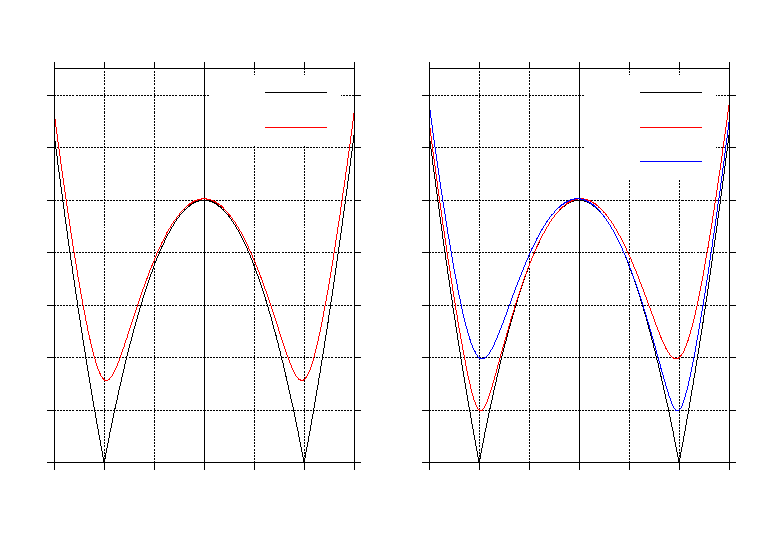
\includegraphics{Figures/twowires/Dispersionexamples/kdepend}}%
    \gplfronttext
  \end{picture}%
\endgroup
  
\caption{The energy dispersion is plotted in the two cases: imaginary and real interwire pairing, $\Delta^{12}_k$. When both pairings are zero, we simply get $|\varepsilon_k|$ shown in black. Left figure, imaginary interwire pairing: in red: $E^{\pm}_{F,k} = \sqrt{\varepsilon^2_k + \left(\Delta^{11}_k\right)^2 + \left|\Delta^{12}_k\right|^2}$. The dispersions are completely degenerate. Right figure, real interwire pairing: In red: $E^{+}_{F,k}$. In blue: $E^{-}_{F,k}$. The dispersions, $E^{\pm}_{F,k} = \sqrt{\varepsilon_k^2 + \left(\Delta^{11}_k \pm \Delta^{12}_k\right)^2}$, are only degenerate in $k = 0$. Notice, that $E^{+}_{F,-k} = E^{-}_{F,k}$. We have set: $\mu / \epsilon_{F,0} = 1$, $\Delta^{11}_k / \epsilon_{F,0} = 0.3 k / k_F$ linear, and $\Delta^{12}_k / \epsilon_{F,0} = 0.1$ constant. }  
\label{fig.Dispersionexamples}  
\end{center}    
\end{figure}

We now describe the diagonalisation in more detail. The new quasiparticle operators are found by finding the eigenvectors to $\mathcal{H}_{FF,k}$. We define the quasiparticle fermionic operators $\gamma_{j,k}$ by:
\begin{equation}
\begin{bmatrix} c_{1,k} \\ c^\dagger_{1,-k} \\ c_{2,k} \\ c^\dagger_{2,-k} \end{bmatrix} = U_{F,k}\begin{bmatrix} \gamma_{1,k} \\ \gamma^{\dagger}_{1,-k} \\ \gamma_{2,k} \\ \gamma^{\dagger}_{2,-k} \end{bmatrix}.
\label{eq.zetaoperatorstwowiresdefinition}
\end{equation} 
The $\gamma$-operators have to obey the same anticommutation relations as the $c$-operators. Specifically, all anticommutators between 1 and 2 quasiparticles, like $\{\gamma_1, \gamma_2 \} $, vanish. $\mathcal{H}_{FF,k}$ should then be diagonalised to yield:
\begin{equation}
U^\dagger_{FF,k}\mathcal{H}_{FF,k}U_{FF,k} = \begin{bmatrix} 
E^{-}_{F,k} & 0        & 0       & 0        \\ 
0       & -E^{-}_{F,-k} & 0       & 0        \\ 
0       & 0        & E^{+}_{F,k} & 0        \\ 
0       & 0        & 0       & -E^{+}_{F,-k} \\ 
\end{bmatrix} = \begin{bmatrix} 
E^{-}_{F,k} & 0        & 0       & 0        \\ 
0       & -E^{+}_{F,k} & 0       & 0        \\ 
0       & 0        & E^{+}_{F,k} & 0        \\ 
0       & 0        & 0       & -E^{-}_{F,k} \\ 
\end{bmatrix} \nonumber
\end{equation}
Further the diagonalisation must respect the symmetry in the 1 and 2 fermions of the Hamiltonian. Specifically the assumption of $\Delta^{22}_k = -\Delta^{11}_k$ must be selfconsistent. From equation \ref{eq.intrawirepairingpotentialdef} this means that $\braket{c_{2,k}c_{2,-k}} = -\braket{c_{1,k}c_{1,-k}}$. Finally, since the elements of $C_k$ are not independent, we get some internal structure of $U_{F,k}$. Let us write the elements of $U_{F,k}$ as $u^{ij}_k$. From equation \eqref{eq.zetaoperatorstwowiresdefinition} we take the first row and the conjugate of the second row with $-k \to k$:
\begin{align}
c_{1,k} &= u^{11\phantom{*}}_{+k} \gamma_{1,k} + u^{12\phantom{*}}_{+k} \gamma^\dagger_{1,-k} + u^{13\phantom{*}}_{+k} \gamma_{2,k} + u^{14\phantom{*}}_{+k} \gamma^\dagger_{2,-k}, \nonumber \\
c_{1,k} &= u^{22*}_{-k} \gamma_{1,k} + u^{21*}_{-k} \gamma^\dagger_{1,-k} + u^{24*}_{-k} \gamma_{2,k} + u^{23*}_{-k} \gamma^\dagger_{2,-k}. \nonumber
\end{align}
Since the coefficients in front of e.g. $\gamma_{1,k}$ must be the same in both expressions, we get that $u^{11}_{+k} = u^{22*}_{-k}$. This restriction stems from the fact that the elements of the Nambu spinor $C_k$ are not independent. In chapter \ref{Chapter5} we will see that this is described by a built-in particle-hole symmetry, i.e. a symmetry between $c$ and $c^\dagger$ operators. $U_{F,k}$ thus has the following structure:
\begin{equation}
U_{F,k} = \begin{bmatrix} 
u^{22*}_{-k} & u^{21*}_{-k} & u^{24*}_{-k} & u^{23*}_{-k}           \\  
u^{21}_k 	 & u^{22}_k 	& u^{23}_k 	   & u^{24}_k               \\ 
u^{42*}_{-k} & u^{41*}_{-k} & u^{44*}_{-k} & u^{43*}_{-k}           \\ 
u^{41}_k 	 & u^{42}_k 	& u^{43}_k 	   & u^{44}_k
\end{bmatrix}. \nonumber
\end{equation}
Now define the norms $A^{\pm}_k = 2 \sqrt{ E^{\pm}_{F,k}(\varepsilon_k + E^{\pm}_{F,k}) }$. With a bit of trial and error the above requirements combined result in:
\begin{equation}
U_{F,k} = \begin{bmatrix} 
\frac{\varepsilon_k + E^{-}_{F,k}}{A^{-}_k}    & -\frac{\Delta^{11}_k + \Delta^{12}_k}{A^{+}_k} & \frac{\varepsilon_k + E^{+}_{F,k}}{A^{+}_k}     & -\frac{\Delta^{11}_k - \Delta^{12}_k}{A^{-}_k}  \\  
\frac{\Delta^{11}_k - \Delta^{12*}_k}{A^{-}_k} & \frac{\varepsilon_k + E^{+}_{F,k}}{A^{+}_k}    & \frac{\Delta^{11}_k + \Delta^{12*}_k}{A^{+}_k}  & \frac{\varepsilon_k + E^{-}_{F,k}}{A^{-}_k}     \\ 
-\frac{\varepsilon_k + E^{-}_{F,k}}{A^{-}_k}   & -\frac{\Delta^{11}_k + \Delta^{12}_k}{A^{+}_k} & \frac{\varepsilon_k + E^{+}_{F,k}}{A^{+}_k}     & \frac{\Delta^{11}_k - \Delta^{12}_k}{A^{-}_k} \\ 
\frac{\Delta^{11}_k - \Delta^{12*}_k}{A^{-}_k} & -\frac{\varepsilon_k + E^{+}_{F,k}}{A^{+}_k}   & -\frac{\Delta^{11}_k + \Delta^{12*}_k}{A^{+}_k} & \frac{\varepsilon_k + E^{-}_{F,k}}{A^{-}_k} 
\end{bmatrix}. \nonumber
\end{equation}
The diagonalisation of the Hamiltonian is now straight forward. $U^\dagger_{F,k}\mathcal{H}_{FF,k}U_{F,k}$ is diagonal with the eigenvalues $+E^{\pm}_{F,k}$ and $-E^{\pm}_{F,k}$ alternating in the diagonal as shown above. The result of the diagonalisation is therefore:
\begin{align}
H_{FF} &= \Phi + \sum_{k} \left[ E^{-}_{F,k}\gamma^\dagger_{1, k}\gamma_{1, k} + E^{+}_{F,k}\gamma^\dagger_{2, k}\gamma_{2, k} \right], \nonumber \\ 
\Phi &= \tilde{\Phi} - \frac{1}{2}\sum_k \left[ E^{-}_{F,k} + E^{+}_{F,k} \right], 
\label{eq.2wiresDiagonalisedHamiltonian}
\end{align}  
Here we have defined the ground state energy relative to the chemical potential, $\Phi$. Thus the ground state of the system at $T = 0$ is defined by having no quasiparticles present: $\gamma_{j,k} \ket{\text{S}}_0 = 0$ for all $k$.\footnote{S is short for \text{S}uperfluid ground state.} This means we can write the ground state as:
\begin{equation}
\ket{\text{S}}_0 \propto \prod_{j,k > 0} \gamma_{j,-k}\gamma_{j,k}\ket{0}.
\label{eq.superfluidgroundstate}
\end{equation}
If one inserts the transformation to the regular fermionic $c$-operators, terms like $c^\dagger_{1,-k}c^\dagger_{1,k}$ appear. This is a manifestation of the concept of Cooper pairs: in the ground state all the fermions are in pairs with opposite momenta. The excited states consequently consists of breaking up a number of Coopers pairs: $\gamma^\dagger_{j,k}\ket{\text{S}}_0$. The energy of such excitations is $E^{\pm}_{F,k}$ with the minus for $j = 1$ and the plus for $j = 2$. These excitations consist of a superposition of particles and holes as is evident from the form of $U_{F,k}$. 

From the diagonalisation we can also find the distribution of the quasiparticles, $\braket{\gamma^\dagger_{j,k}\gamma_{j,k}}$. Since the presence of such a particle is a fermionic excitation with energy $E^{\pm}_{F,k}$ it is intuitively clear that they are distributed according to the Fermi-Dirac distribution given by:
\begin{equation}
\braket{\gamma^\dagger_{j,k} \gamma_{j,k}} = f(E^{\pm}_{F,k}) = \frac{1}{\text{e}^{\beta E^{\pm}_{F,k}} + 1}, 
\label{eq.Distribution.quasiparticles}
\end{equation}
where the minus is for $j = 1$, the plus for $j = 2$. Notice the absence of a quasiparticle chemical potential. This is because the number of quasiparticles is not fixed. One can show this with a standard statistical mechanics argument, see e.g. \cite[p. 225]{SchroederThermal}. For a rigorous argument based on the second quantized operators, the reader is referred to appendix \ref{Appendix.distribution.quasiparticles}. Because of the absence of a quasiparticle chemical potential the distribution function differs functionally from the distribution of the fermions in the free gas. In the free gas for low temperatures, the distribution is close to one for $|k|< \sqrt{2m_F\mu}$ and quickly decays to zero outside this region. The present quasiparticle distribution is exactly zero for $T = 0$ and exhibit well-defined peaks around $k = \pm \sqrt{2m_F\mu}$ for $T > 0$ showing that the excitations are near the Fermi points of the free gas. 

The expected temperature dependence of the system is inferred from the original BCS-theory \cite[chapter 3]{Tinkham}. The pairing potentials $\Delta^{ij}_k(T)$ are expected to have their maximum for $T = 0$ and then monotonically decrease to 0, when the temperature is increased to a critical temperature $T_c$. If either $\Delta^{11}_k$ or $\Delta^{12}_k$ is nonzero, we will see that $E^{\pm}_{F,k} = \sqrt{\varepsilon_k^2 + |\Delta^{11}_k \pm \Delta^{12}_k|^2} > 0$ for all $k$. In turn we get $\min_k[E^{\pm}_{F,k} / k] > 0$ which is exactly Landau's criterion for superfluidity \cite[pp. 88-90]{LandauStatPhys2}. Explicitly this means that if the gas of fermions move with a speed below $v_c = \min_k[E^{\pm}_{F,k} / k] > 0$, the gas will not experience any drag. Hence, it is a superfluid. If we increase the temperature across $T_c$, the system will therefore experience a phase transition from a superfluid phase below $T_c$ to a normal phase above $T_c$.

In terms of Landau's theory of phase transitions as reviewed in section \ref{sec.landauphasetransitions} the order parameters are the quantities that are zero in the normal phase above the critical temperature, $T_c$, and nonzero below. From this it is clear that $\braket{c_{i,-k}c_{j,k}}$, or equivalently $\Delta^{ij}_k$, are exactly the order parameters of the system.

As noted in the derivation of BCS Hamiltonian, it does not conserve the number of fermions: $[N_{j,F}, H_{FF}] \neq 0 $, where $N_{j,F} = \sum_k c^\dagger_{j,k} c_{j,k}$ is the number operator for fermions in wire $j = 1, 2$. In appendix \ref{Appendix.fermionnumberfluctuation}, we show that within the BCS treatment the fluctuation in the number of fermions is $\propto 1 / N_F$ and small. In this sense we consider the number of fermions not conserved but well-defined in the thermodynamic limit. We will from now on therefore use $N_F$ both for the number operator and the mean value $\braket{N_F}$. It should be clear from the context which one is meant.

\section{Gap and number equations} \label{sec.gapandnumberequations}
In this section we derive self-consistency equations for the pairing and chemical potentials, known as the gap and number equations. Since we use a BCS approach, we collectively refer to these equations as the \textit{BCS} equations. Again, this calculation is straightforward when the diagonalisation is in place, but lengthy due to the $4 \times 4$ problem at hand. 

Inspecting the definitions of the pairing potentials in equations \eqref{eq.intrawirepairingpotentialdef} and \eqref{eq.interwirepairingpotentialdef} we see that we need to calculate the mean fields $\braket{ c_{i, k} c_{j,-k} }$. We will do this in detail for $\braket{c_{1,k}c_{1,-k}}$ to see how the computation plays out. We write $c_{1,k} = u^{11}_{k} \gamma_{1,k} + u^{12}_{k} \gamma^\dagger_{1,-k} + u^{13}_{k} \gamma_{2,k} + u^{14}_{k} \gamma^\dagger_{2,-k}$, with $u^{ij}_k$ the elements of $U_{F,k}$. Then:
\begin{equation}
\braket{c_{1,k}c_{1,-k}} = u^{11}_{k}u^{12}_{-k}\braket{\gamma_{1,k}\gamma^\dagger_{1,k}} + u^{12}_{k}u^{11}_{-k}\braket{\gamma^\dagger_{1,-k}\gamma_{1,-k}} + u^{13}_{k}u^{14}_{-k}\braket{\gamma_{2,k}\gamma^\dagger_{2,k}} + u^{14}_{k}u^{13}_{-k}\braket{\gamma^\dagger_{2,-k}\gamma_{2,-k}}, \nonumber
\end{equation}
where we use that the only nonzero thermal averages are on the form $\braket{\gamma_{j,k}\gamma^\dagger_{j,k}}$ or $\braket{\gamma^\dagger_{j,k}\gamma_{j,k}}$. Using that the quasiparticles are distributed according to the Fermi-Dirac distribution, equation \eqref{eq.Distribution.quasiparticles}, we get:
\begin{equation}
\braket{c_{1,k}c_{1,-k}} = \frac{\Delta^{11}_k + \Delta^{12}_k}{4E^{+}_{F,k}}\left(1 - 2f(E^{+}_{F,k})\right) + \frac{\Delta^{11}_k - \Delta^{12}_k}{4E^{-}_{F,k}}\left(1 - 2f(E^{-}_{F,k})\right). 
\label{eq.meanfield11}
\end{equation}
Calculating $\braket{c_{2,k}c_{2,-k}}$ gives exactly minus the above. Hence, the assumption $\braket{c_{2,k}c_{2,-k}} = -\braket{c_{1,k}c_{1,-k}}$ is self-consistent. An analogous calculation for $\braket{c_{2,k}c_{1,-k}}$ yields:
\begin{equation}
\braket{c_{2,k}c_{1,-k}} = \frac{\Delta^{12}_k + \Delta^{11}_k}{4E^{+}_{F,k}}\left(1 - 2f(E^{+}_{F,k})\right) + \frac{\Delta^{12}_k - \Delta^{11}_k}{4E^{-}_{F,k}}\left(1 - 2f(E^{-}_{F,k})\right). 
\label{eq.meanfield12}
\end{equation}
Plugging these mean fields into the definition of the pairing potentials, equations \eqref{eq.intrawirepairingpotentialdef} and \eqref{eq.interwirepairingpotentialdef}, we get the gap equations:
\begin{align}
\Delta^{11}_k &= -\frac{1}{\mathcal{L}}\sum_{k'} W_{\text{ind}}^{11}(k, k')\frac{\Delta^{11}_{k'} + \Delta^{12}_{k'}}{2E^{+}_{F,k'}}\tanh\left[\frac{\beta E^{+}_{F,k'}}{2}\right], \nonumber \\
\Delta^{12}_k &= -\frac{1}{\mathcal{L}}\sum_{k'} W_{\text{ind}}^{12}(k, k')\frac{\Delta^{12}_{k'} + \Delta^{11}_{k'}}{2E^{+}_{F,k'}}\tanh\left[\frac{\beta E^{+}_{F,k'}}{2}\right].
\label{eq.2wiresgapequations}
\end{align}
Here the oddness of $\Delta^{11}_k$ and evenness of $\Delta^{12}_k$ have been used to simplify the expressions. We have used that $1 - 2f(E) = \tanh\left[\frac{\beta E}{2}\right]$ with inverse temperature $\beta = 1 / k_BT$. Finally, we have defined the \textit{inter}wire effective interaction $W_{\text{ind}}^{12}(k, k')$ to make the equations symmetric:
\begin{equation}
W_{\text{ind}}^{12}(k, k') = \frac{1}{2}\left[V_{\text{ind}}^{12}(k - k', 0) + V_{\text{ind}}^{12}(k + k', 0) \right].
\label{eq.EffectiveInteraction.interwire}
\end{equation}
This definition is completely analogous to the definition of the intrawire effective interaction, see equation \eqref{eq.EffectiveInteraction.intrawire}. 

Now we wish to calculate the number equation $N_F = \sum_k \braket{c^\dagger_{j,k}c_{j,k}}$, hence we need the thermal average of $\braket{c^\dagger_{j,k}c_{j,k}}$. The calculation is carried through in complete analogy to the above, resulting in:
\begin{equation}
\braket{c^\dagger_{j,k}c_{j,k}} = \frac{1}{4}\left( 1 - \frac{\varepsilon_k}{E^{+}_{F,k}}\tanh\left[\frac{\beta E^{+}_{F,k}}{2}\right] \right) + \frac{1}{4}\left( 1 - \frac{\varepsilon_k}{E^{-}_{F,k}}\tanh\left[\frac{\beta E^{-}_{F,k}}{2}\right] \right).
\label{eq.meanoccupancy}
\end{equation}
This is the mean occupancy of the $k$'th momentum state in wire $j$. It is seen to be independent of the wire. Plugging it into the number equation and transforming the sum to an integral gives us the number equation:
\begin{equation}
n_F = \frac{1}{2}\int \frac{dk}{2\pi} \left( 1 - \frac{\varepsilon_k}{E^{+}_{F,k}}\tanh\left[\frac{\beta E^{+}_{F,k}}{2}\right] \right). 
\label{eq.2wiresnumberequation}
\end{equation}
The BCS equations have thus been derived. The real part of the first gap equation, the real and imaginary part of the second one and the number equation gives us four equations for the four quantitites $\Delta^{11}_k, \Delta^{12}_{k,r}, \Delta^{12}_{k,i} $ and $\mu$. Here we write the interwire pairing as decomposed in its real and imaginary parts: $\Delta^{12}_k = \Delta^{12}_{k,r} + i\Delta^{12}_{k,i}$. Finally, taking the imaginary part of the first gap equation gives a fifth self-consistency equation:
\begin{equation}
0 = -\frac{1}{\mathcal{L}}\sum_{k'} W_{\text{ind}}^{11}(k, k')\frac{\Delta^{12}_{k',i}}{2E^{+}_{F,k'}}\tanh\left[\frac{\beta E^{+}_{F,k'}}{2}\right].
\end{equation}
This equation has two trivial solutions. The first is, where the interwire pairing is real. Then the integrand is 0 and the equation is fulfilled. The second is, where the interwire pairing is purely imaginary. Then the two dispersion relations are identical: $E^{\pm}_{F,k} = \sqrt{\varepsilon_k^2 + (\Delta^{11}_k)^2 + |\Delta^{12}_k|^2}$. The summand is therefore an odd function in $k'$ and so the equation is again fulfilled. We will only investigate these two cases, because they exhibit interesting symmetries of the system. This is discussed in chapter \ref{Chapter5}. 

Physically, the BCS equations \eqref{eq.2wiresgapequations} and \eqref{eq.2wiresnumberequation} express that the pairings and chemical potentials adjust to each other. If for example the intrawire pairing, $\Delta^{11}_k$, is changed, the interwire pairing, $\Delta^{12}_k$, changes accordingly, equation \eqref{eq.2wiresgapequations}. Further, the chemical potential changes to keep the number of fermions fixed, equation \eqref{eq.2wiresnumberequation}. This also gives us a way of determining the functions numerically in a simple manner. We plug in a start guess for the pairing and chemical potentials. This gives an updated version of the potentials which are reinserted into the equations. This process is repeated, until the potentials have converged. This numerical analysis is performed in chapter \ref{Chapter6}. Before moving on to the symmetries and topology of the system, we derive an expression for the ground state energy.

\section{Ground state energy} \label{sec.groundstateenergy}
An explicit expression for the ground state energy relative to the chemical potential, $\Phi$, from equation \eqref{eq.2wiresDiagonalisedHamiltonian} is derived similarly to the gap equations of the previous section. For $T = 0$ the expression is particularly simple. We get:
\begin{equation}
\frac{\Phi}{\epsilon_{F,0} N_F} = -\frac{1}{4} \int d\tilde{k} \frac{(\tilde{\varepsilon}_{\tilde{k}} - \tilde{E}^{+}_{F, \tilde{k}})^2}{\tilde{E}^{+}_{F, \tilde{k}}}, \hspace{0.5cm} T = 0. 
\label{eq.2wiresGrandGroundStateEnergy}
\end{equation}
We have expressed the momentum as $\tilde{k} = k / k_F$, and the energies as $\tilde{E} = E / \epsilon_{F,0}$. We notice that $\Phi$ is negative. This is simply, because $\Phi$ is the energy relative to the chemical potential, the so-called grand potential. The motivation for calculating this is the following. For any temperature the grand potential, $\Phi$, is given by $\Phi = E_0 - TS - 2\mu N_F = F - 2\mu N_F$, where $F$ is the Helmholtz free energy \cite[pp. 161-162]{SchroederThermal}. The presence of the factor of 2 is simply because there are $N_F$ fermions in \textit{each} wire. Physically, we will hold the number of particles fixed. This means that it is the Helmholtz free energy $F = \Phi + 2\mu N_F$ we have to minimize to find the preferred state, not $\Phi$. We will focus on the $T = 0$ case. Hence, the aim is to calculate the ground state energy $E_0 = \Phi + 2\mu N_F$ as a function of the interwire distance, $d$, for the two interesting cases: $\Delta^{12}_k$ real and imaginary. The one which exhibits the minimal energy is the energetically favourable state. 


